\documentclass[12pt]{article}
\usepackage[T1]{fontenc}
\usepackage[T1]{polski}
\usepackage[cp1250]{inputenc}
\newcommand{\BibTeX}{{\sc Bib}\TeX} 
\usepackage{graphicx}
\usepackage{amsfonts}
\usepackage{float}

\setlength{\textheight}{21cm}

\title{{\bf Zadanie nr 4 - Przeksztalcenie Fouriera, Walsha-Hadamarda, kosinusowe i falkowe,szybkie algorytmy}\linebreak
Cyfrowe Przetwarzanie Sygna�u}
\author{Justyna Hubert, 210200 \and Karol Podlewski, 210294}
\date{19.05.2019}

\begin{document}
\clearpage\maketitle
\thispagestyle{empty}
\newpage
\setcounter{page}{1}


%%%%%%%%%%%%%%%%%%%%%%%%%%%%%%%%%%%%%%%%%%%%%%%%%%%%%%%%%%%%
%% CEL ZADANIA
%%%%%%%%%%%%%%%%%%%%%%%%%%%%%%%%%%%%%%%%%%%%%%%%%%%%%%%%%%%%
\section{Cel zadania}
Celem cwiczenia jest zapoznanie sie z operacjami transformacji sygnal�w dyskretnychprzy u�yciu wybranych metod.
%%%%%%%%%%%%%%%%%%%%%%%%%%%%%%%%%%%%%%%%%%%%%%%%%%%%%%%%%%%%
%% WSTEP TEORETYCZNY
%%%%%%%%%%%%%%%%%%%%%%%%%%%%%%%%%%%%%%%%%%%%%%%%%%%%%%%%%%%%
\section{Wstep teoretyczny}
Jest to usprawniony program z zadania 1, 2 oraz 3, dostosowany do instrukcji z zadania czwartego ~\cite{instrukcja}. \\

W ramach cwiczenia nale�alo dodac mo�liwosc odczytu i zapisu sygnal�w o wartosciach zespolonych, umo�liwic rysowanie wykres�w sygnal�w dyskretnych o wartosciach zespolonych w postaci dw�ch wykres�w o wsp�lnej dziedzinie ulo�onych jeden nad drugim. Przyjeto, �e sygnaly zespolone beda tylko wynikiem transformacji Fouriera, a co za tym idzie beda prezentowac funkcje w dziedzinie czestotliwosci. Dostepne mialy byc tak�e dwa atrybuty prezentacji wykresu:

\begin{itemize}
	\item (W1) - g�rny   wykres   prezentuje   czesc   rzeczywista   amplitudy   w   funkcji czestotliwosci, a wykres dolny czesc urojona,
	\item (W2) - g�rny wykres prezentuje modul liczby zespolonej, a dolny argument liczbywfunkcji czestotliwosci
\end{itemize}

Ponadto, zaimplementowalismy nastepujace transormacje sygnal�w:
\begin{itemize}
	\item (F1) - dyskretna   transformacja   Fouriera   -   algorytm   z   definicji   oraz   szybkatransformacja Fouriera z decymacja w dziedzinie czasu (DIT FFT),
	\item (T3) - transformacja falkowa (jeden poziom), wariant DB8
\end{itemize} 


\pagebreak

%%%%%%%%%%%%%%%%%%%%%%%%%%%%%%%%%%%%%%%%%%%%%%%%%%%%%%%%%%%%
%% SEKCJA EKSPERYMENT�W
%%%%%%%%%%%%%%%%%%%%%%%%%%%%%%%%%%%%%%%%%%%%%%%%%%%%%%%%%%%%
\section{Eksperymenty i wyniki}


\begin{figure}[H]
	\centering
		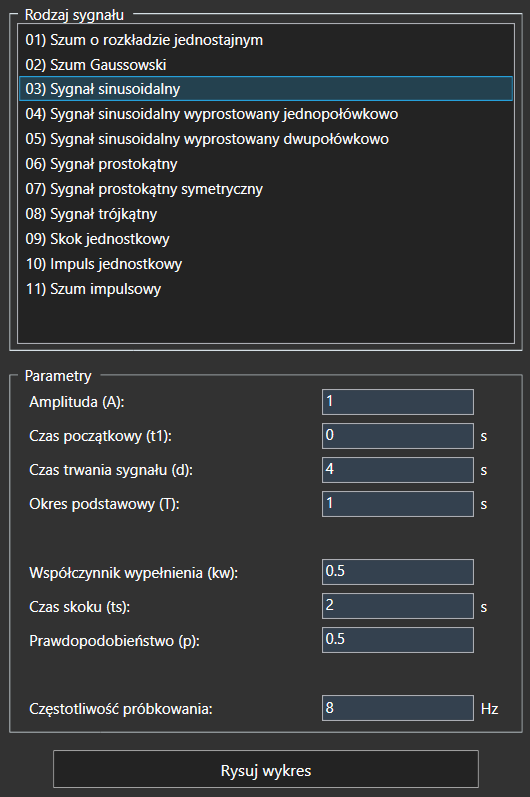
\includegraphics[width=0.7\textwidth]{{Rysunki/SinParam.png}}
	\caption{Parametry, kt�re przyjmowac bedzie wykorzystana przez nas funkcja w eksperymentach.}
\end{figure}

%%%%%%%%%%%%%%%%%%%%%%%%%%%%%%%%%%%%%%%%%%%%%%%%%%%%%%%%%%%%
%%%%%%%%%%%% EKSPERYMENT #1  
\subsection{Dyskretna transormacja Fouriera - algorytm z definicji}

\begin{figure}[H]
	\centering
		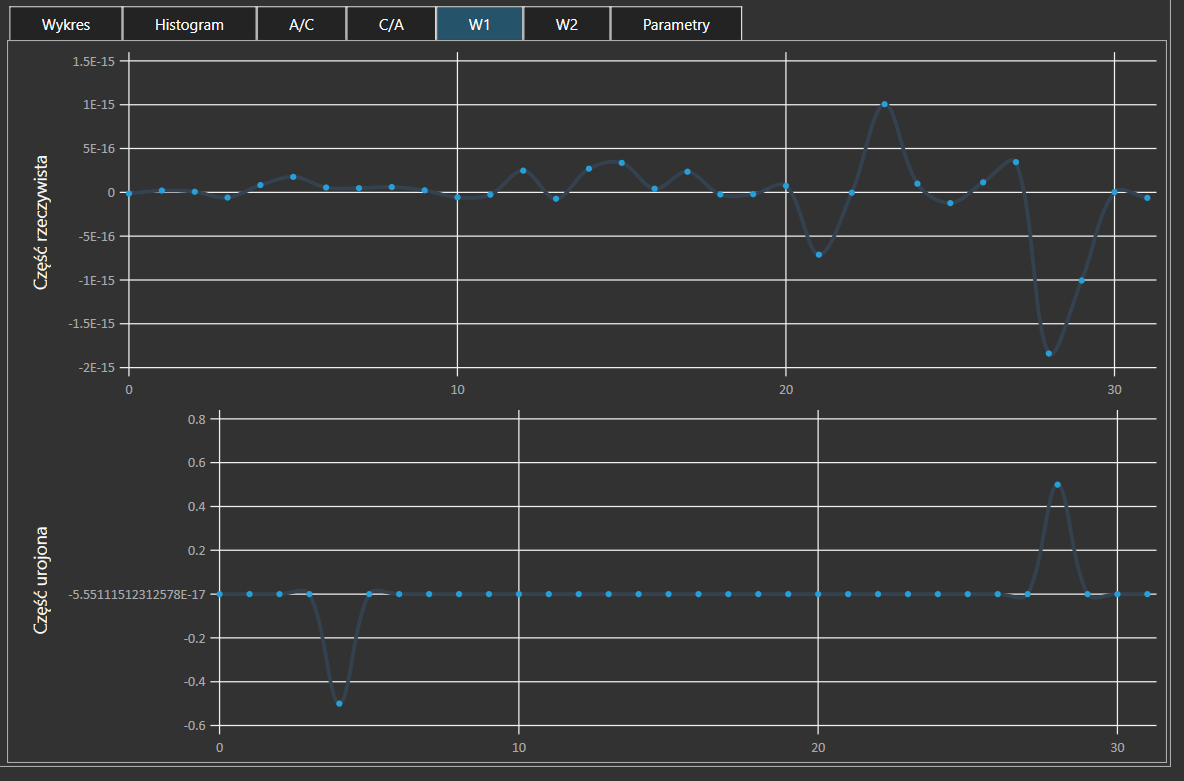
\includegraphics[width=0.7\textwidth]{{Rysunki/FourW1.png}}
	\caption{Dyskretna transformacja Fouriera W1.}
\end{figure}

\begin{figure}[H]
	\centering
		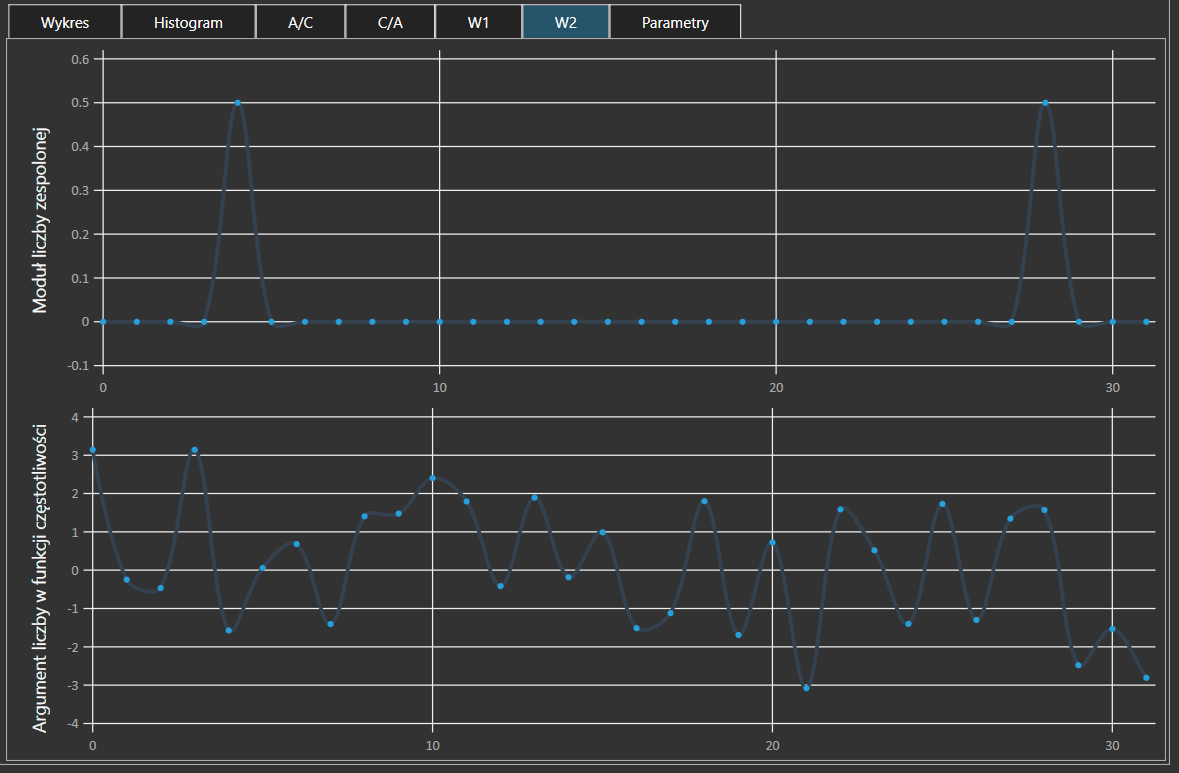
\includegraphics[width=0.7\textwidth]{{Rysunki/FourW2.png}}
	\caption{Dyskretna transformacja Fouriera W2.}
\end{figure}

\begin{figure}[H]
	\centering
		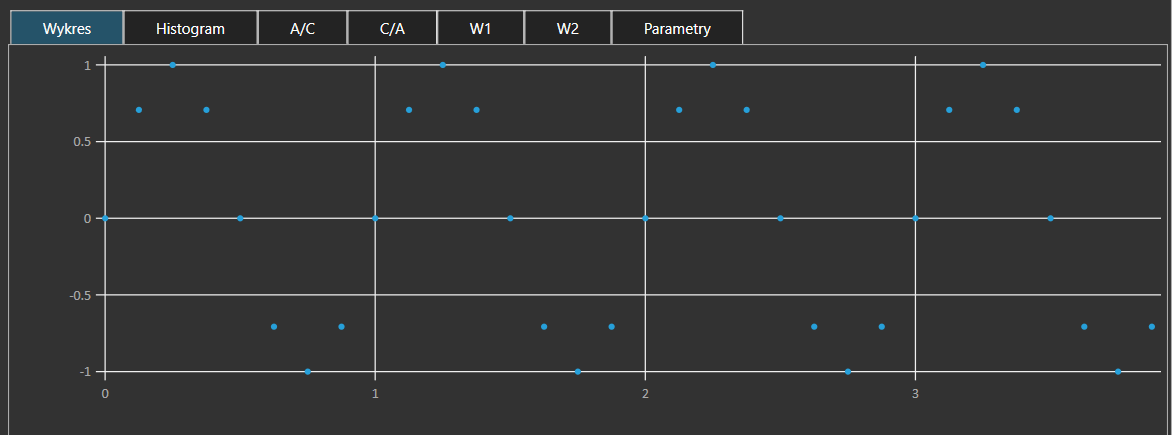
\includegraphics[width=0.7\textwidth]{{Rysunki/FourOdwr.png}}
	\caption{Odwr�cona tranformacja Fouriera.}
\end{figure}


%%%%%%%%%%%%%%%%%%%%%%%%%%%%%%%%%%%%%%%%%%%%%%%%%%%%%%%%%%%%
%%%%%%%%%%%% EKSPERYMENT #2  
\subsection{Szybka transformacja Fouriera z decymacja w dziedzinie czasu}

\begin{figure}[H]
	\centering
		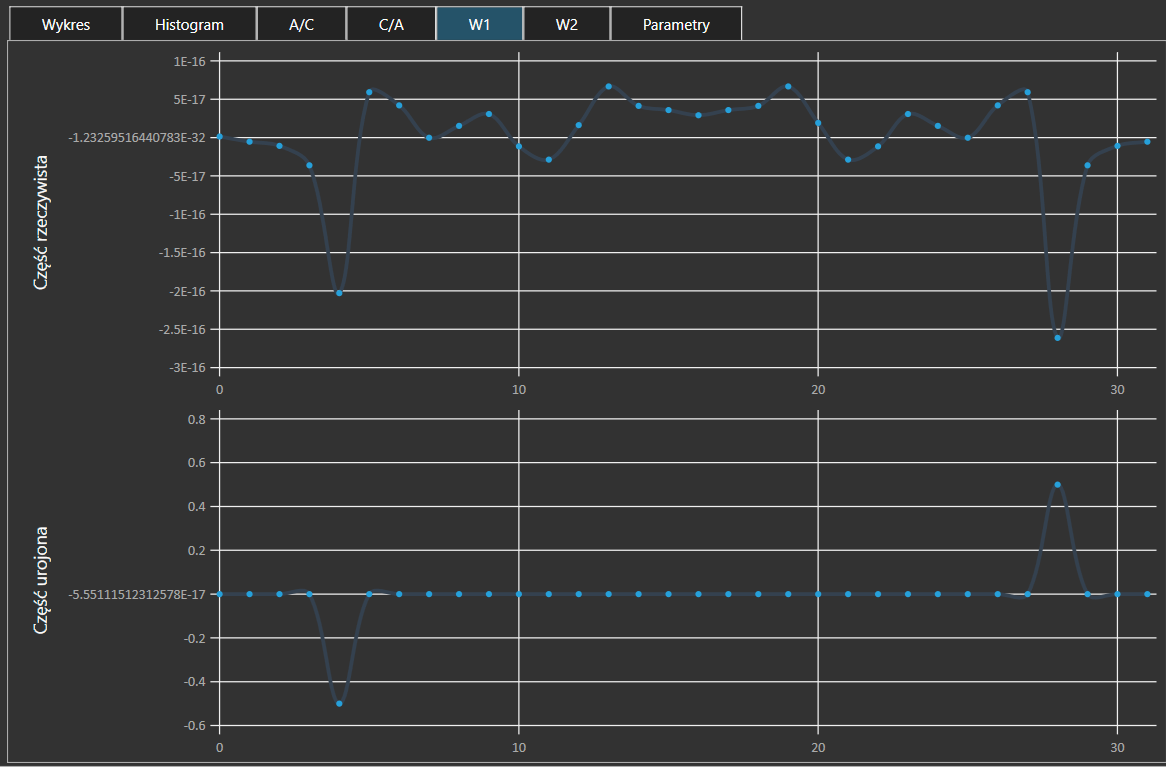
\includegraphics[width=0.7\textwidth]{{Rysunki/SzybFourW1.png}}
	\caption{Szybka transformacja Fouriera W1.}
\end{figure}

\begin{figure}[H]
	\centering
		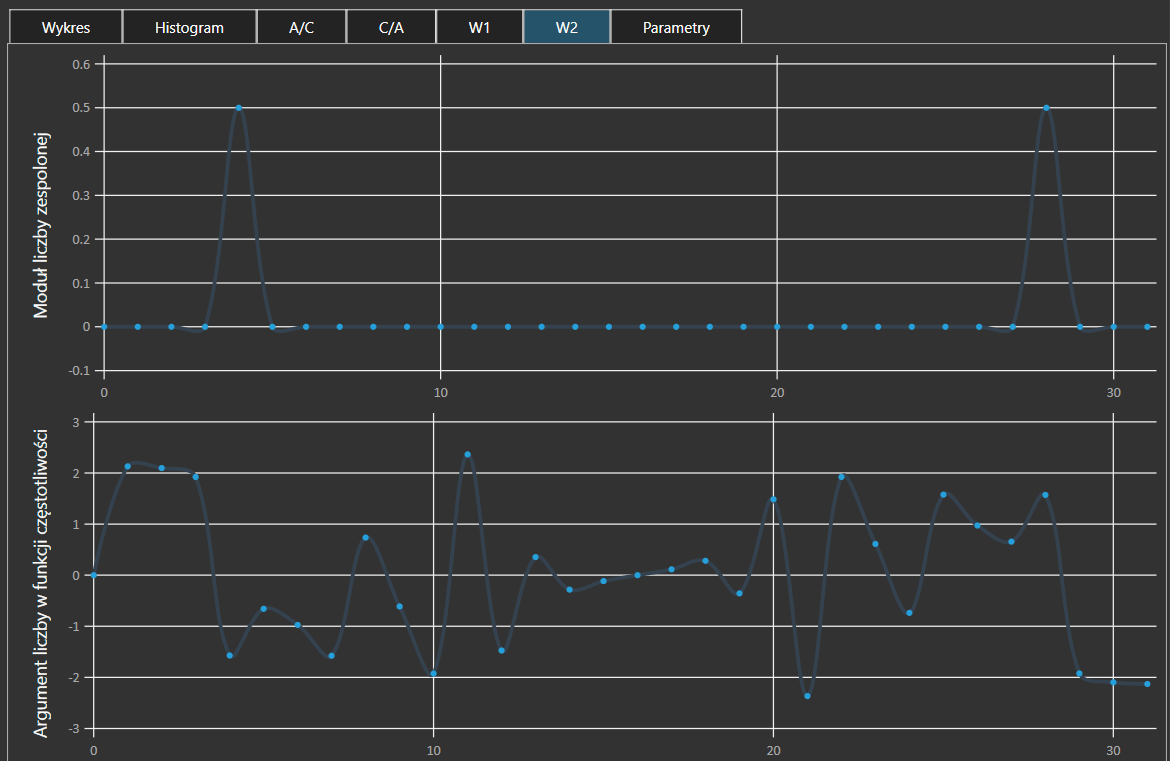
\includegraphics[width=0.7\textwidth]{{Rysunki/SzybFourW2.png}}
	\caption{Szybka transformacja Fouriera W2.}
\end{figure}

\begin{figure}[H]
	\centering
		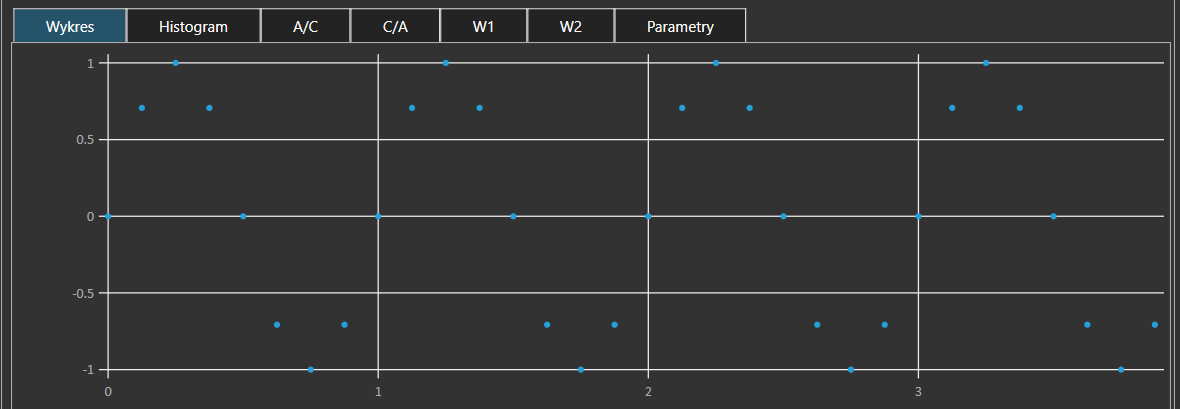
\includegraphics[width=0.7\textwidth]{{Rysunki/SzybFourOdwr.png}}
	\caption{Odwr�cona szybka tranformacja Fouriera.}
\end{figure}

\pagebreak

%%%%%%%%%%%%%%%%%%%%%%%%%%%%%%%%%%%%%%%%%%%%%%%%%%%%%%%%%%%%
%%%%%%%%%%%% EKSPERYMENT #3  
\subsection{Transformacja falkowa wariant DB8} 

\begin{figure}[H]
	\centering
		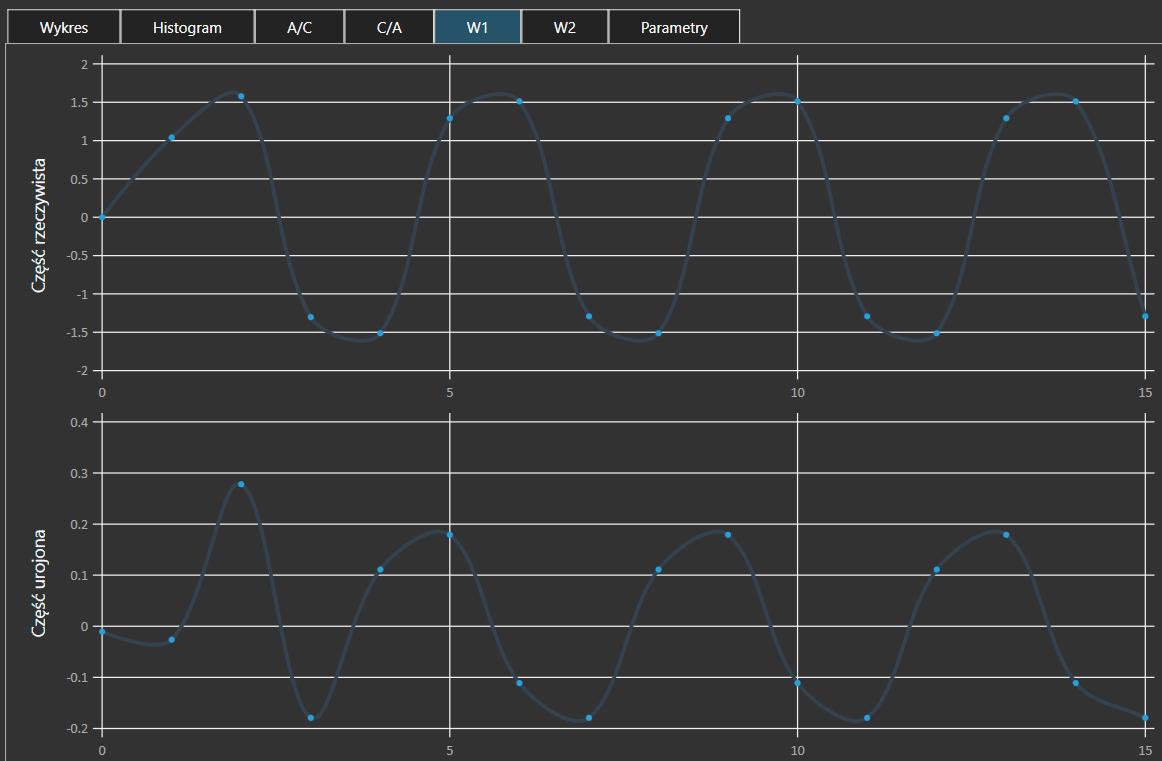
\includegraphics[width=0.7\textwidth]{{Rysunki/FalkW1.png}}
	\caption{Tranformacja falkowa W1.}
\end{figure}

\begin{figure}[H]
	\centering
		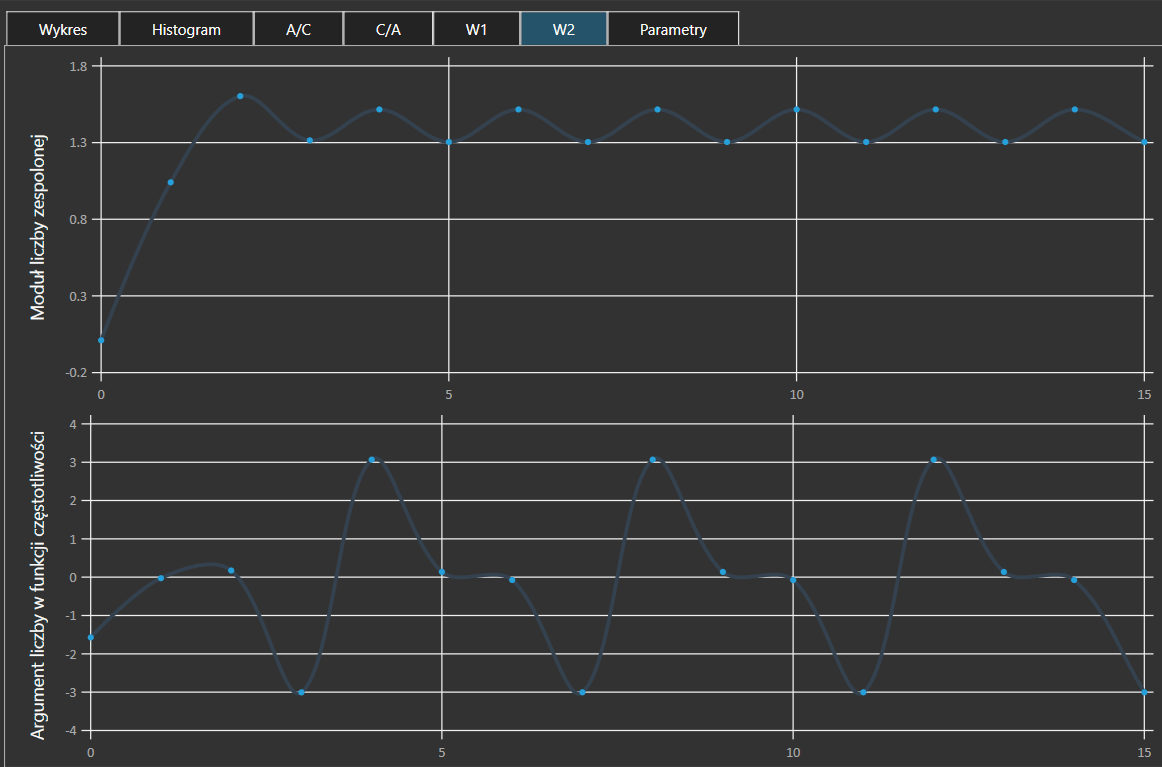
\includegraphics[width=0.7\textwidth]{{Rysunki/FalkW2.png}}
	\caption{Tranformacja falkowa W2.}
\end{figure}

\begin{figure}[H]
	\centering
		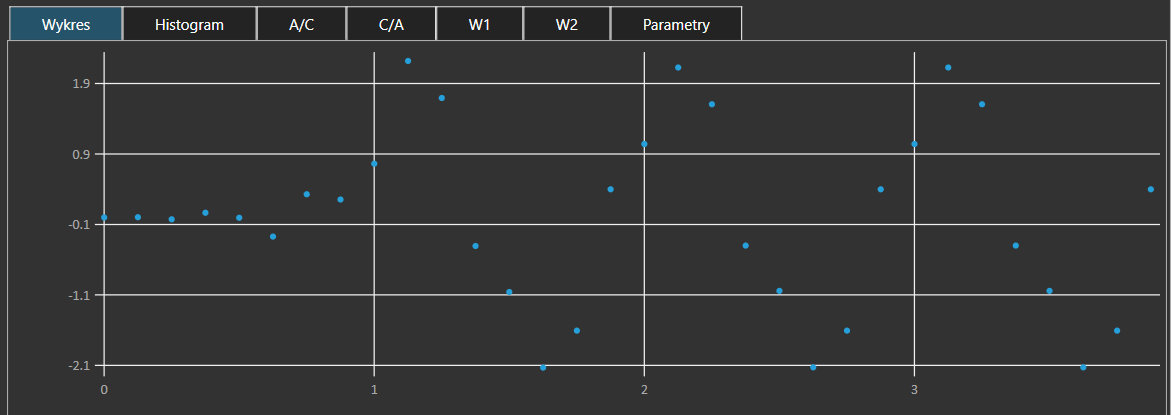
\includegraphics[width=0.7\textwidth]{{Rysunki/FalkOdwr.png}}
	\caption{Transformacja falkowa odwrotna.}
\end{figure}

\pagebreak

%%%%%%%%%%%%%%%%%%%%%%%%%%%%%%%%%%%%%%%%%%%%%%%%%%%%%%%%%%%%
%%%%%%%%%%%% EKSPERYMENT #4  
\subsection{Sygnal dany r�wnaniem S1} 

\begin{figure}[H]
	\centering
		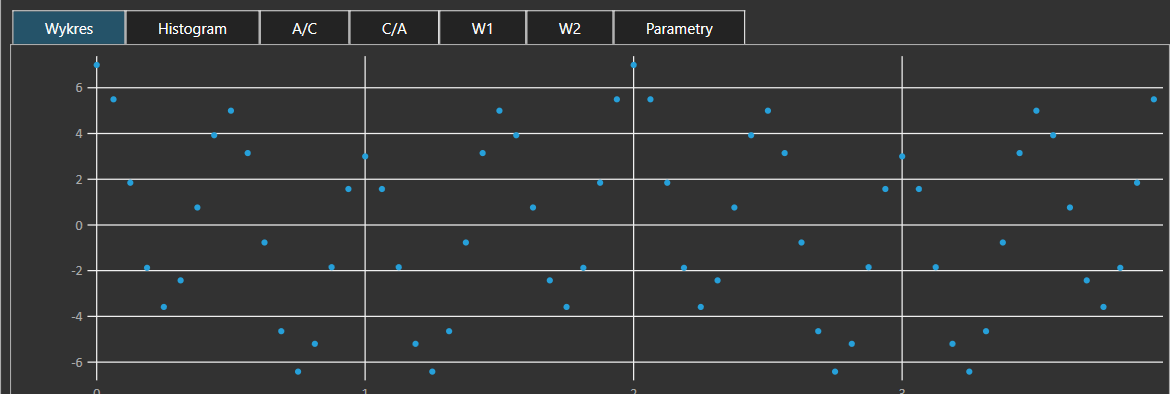
\includegraphics[width=0.7\textwidth]{{Rysunki/S1.png}}
	\caption{Sygnal dany r�wnaniem S1.}
\end{figure}

\begin{figure}[H]
	\centering
		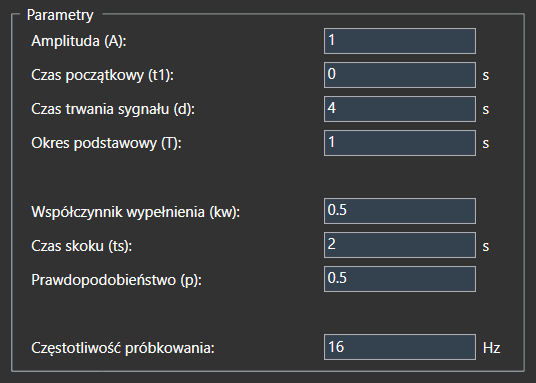
\includegraphics[width=0.7\textwidth]{{Rysunki/S1Param.png}}
	\caption{Parametry r�wnania S1.}
\end{figure}

\begin{figure}[H]
	\centering
		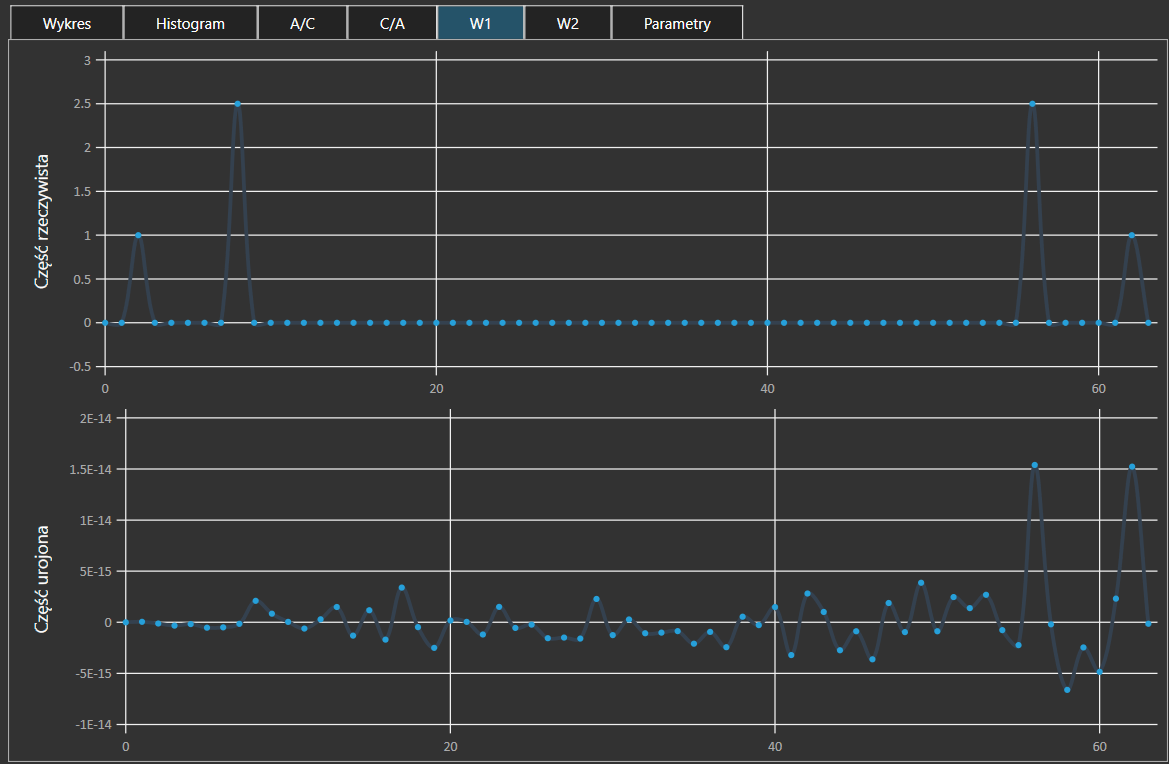
\includegraphics[width=0.7\textwidth]{{Rysunki/S1FourW1.png}}
	\caption{Transformacja dyskretna Fouriera W1.}
\end{figure}

\begin{figure}[H]
	\centering
		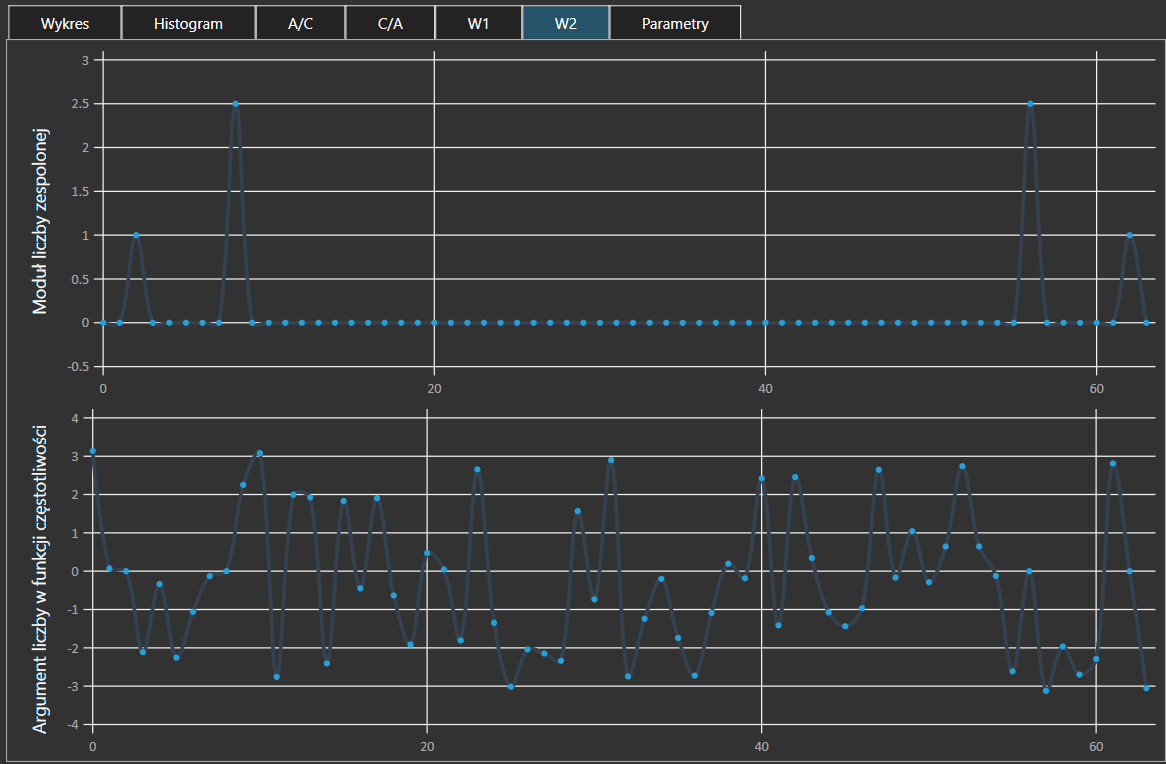
\includegraphics[width=0.7\textwidth]{{Rysunki/S1FourW2.png}}
	\caption{Transformacja dyskretna Fouriera W2.}
\end{figure}

\begin{figure}[H]
	\centering
		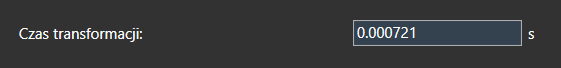
\includegraphics[width=0.7\textwidth]{{Rysunki/S1FourCzas.png}}
	\caption{Czas dyskretnej transformacji Fouriera.}
\end{figure}

\begin{figure}[H]
	\centering
		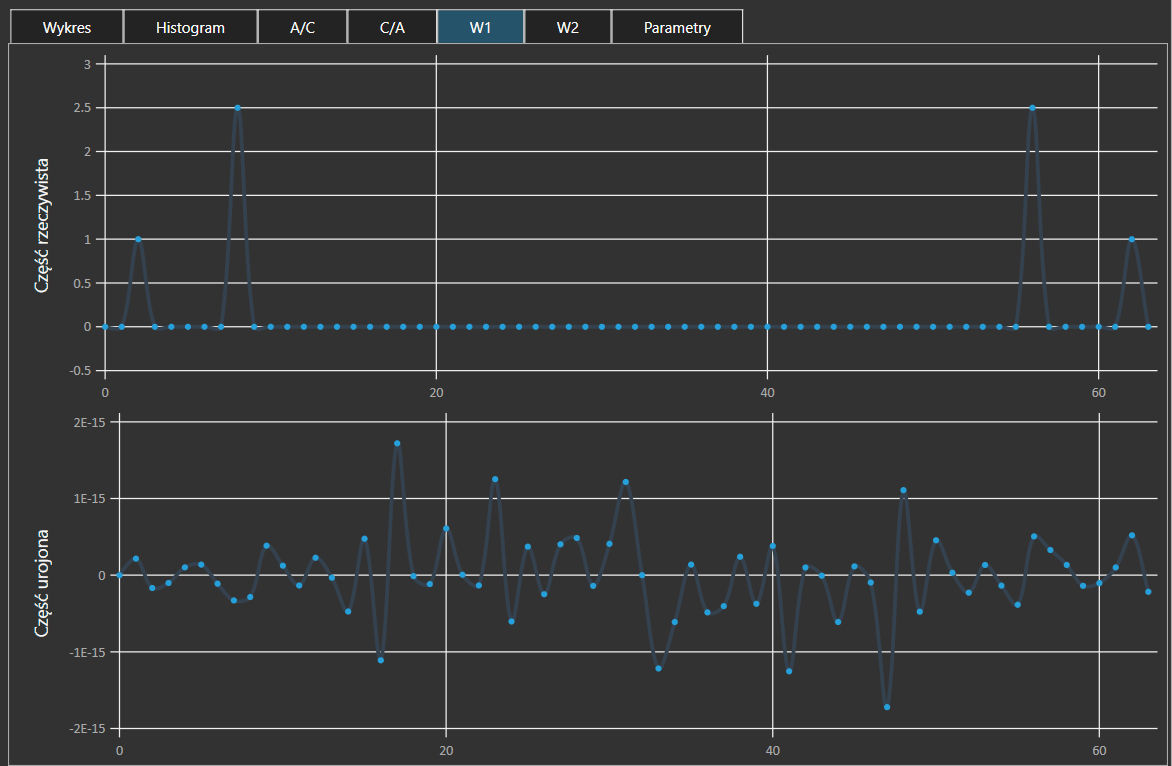
\includegraphics[width=0.7\textwidth]{{Rysunki/S1SzybW1.png}}
	\caption{Szybka transformacja Fouriera W1.}
\end{figure}

\begin{figure}[H]
	\centering
		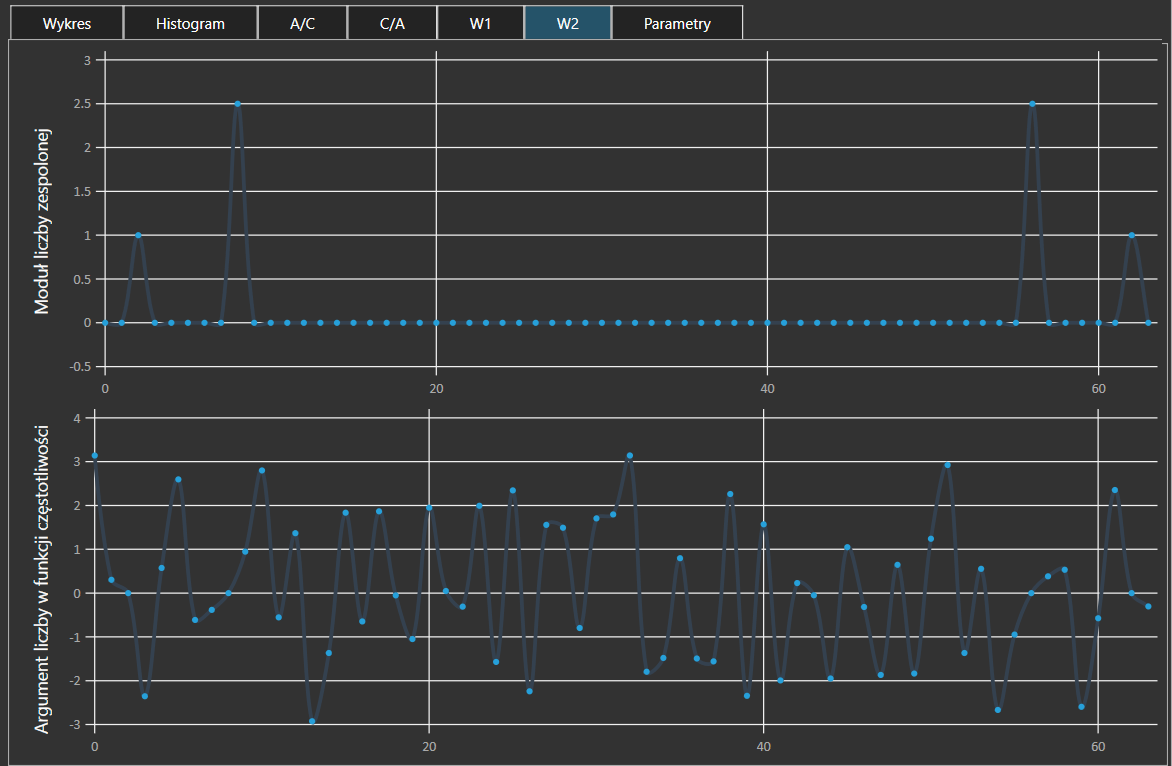
\includegraphics[width=0.7\textwidth]{{Rysunki/S1SzybW2.png}}
	\caption{Szybka transformacja Fouriera W2.}
\end{figure}

\begin{figure}[H]
	\centering
		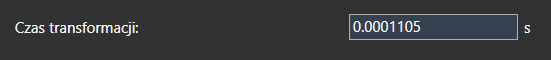
\includegraphics[width=0.7\textwidth]{{Rysunki/S1SzybCzas.png}}
	\caption{Czas szybkiej transformacji Fouriera.}
\end{figure}

\pagebreak

%%%%%%%%%%%%%%%%%%%%%%%%%%%%%%%%%%%%%%%%%%%%%%%%%%%%%%%%%%%%
%% WNIOSKI
%%%%%%%%%%%%%%%%%%%%%%%%%%%%%%%%%%%%%%%%%%%%%%%%%%%%%%%%%%%%
\section{Wnioski}
Aplikacja zostala napisana zgodnie z instrukcj� do zadania ~\cite{instrukcja}. Program poprawnie implementuje dyskretna transformacje Fouriera, szybka transformacje Fouriera z decymacja w dziedzinie czasu oraz transformacje falkowe (wariant DB8). Nasz projekt spelnia wszelkie wymagania opisane w zalo�eniach. 

%%%%%%%%%%%%%%%%%%%%%%%%%%%%%%%%%%%%%%%%%%%%%%%%%%%%%%%%%%%%
%% BIBLIOGRAFIA
%%%%%%%%%%%%%%%%%%%%%%%%%%%%%%%%%%%%%%%%%%%%%%%%%%%%%%%%%%%%
\renewcommand\refname{Bibliografia}
\bibliographystyle{plain}
\bibliography{Zad4_Bibliografia}

\end{document}
